%!TEX program = xelatex
\documentclass[11pt, a4paper]{article}

% AA LINGUA E GESTIONE FONT (Specifica per XeLaTeX)
\usepackage{fontspec}
\setmainfont{Latin Modern Roman}
\usepackage[italian]{babel}

% AA LAYOUT DI PAGINA E TIPOGRAFIA (Ottimizzato per Rilegatura)
\usepackage[left=2.4cm, right=1.6cm, top=2cm, bottom=2cm]{geometry}

% AA Spaziatura tra paragrafi controllata (compatta ed evita salti enormi)
\usepackage[skip=3pt plus 1pt minus 1pt]{parskip}
\setlength{\parindent}{0pt}

% AA Microtype per XeLaTeX
\usepackage[protrusion=true]{microtype}
\raggedbottom

% AA GESTIONE DEI COLORI
\usepackage{xcolor}

% AA MATEMATICA E SIMBOLI
\usepackage{amsmath}
\usepackage{mathtools}
\usepackage{silence}
\usepackage[warnings-off={mathtools-overbracket,mathtools-colon}]{unicode-math}
\setmathfont{Latin Modern Math}

% BB OTTIMIZZAZIONE MATRICI LUNGHE PER LA STAMPA
\setlength{\arraycolsep}{10pt}

% AA Spaziature verticali attorno alle formule matematiche
\setlength{\abovedisplayskip}{3pt plus 1pt minus 1pt}
\setlength{\belowdisplayskip}{3pt plus 1pt minus 1pt}
\setlength{\abovedisplayshortskip}{0pt plus 1pt}
\setlength{\belowdisplayshortskip}{2pt plus 1pt minus 1pt}

% AA GRAFICA ED IMMAGINI
\usepackage{graphicx}
\graphicspath{{./E2_Images/}}
\usepackage{float}

% AA PERSONALIZZAZIONE TITOLI
\usepackage{titlesec}
\titleformat{\section}{\normalfont\Large\bfseries\color{blue!80!black}}{\thesection}{1em}{}
\titleformat{name=\section,numberless}{\normalfont\Large\bfseries\color{blue!80!black}}{}{0pt}{}

\titleformat{\subsection}{\normalfont\large\bfseries}{\thesubsection}{1em}{}
\titleformat{name=\subsection,numberless}{\normalfont\large\bfseries}{}{0pt}{}

\titleformat{\subsubsection}{\normalfont\normalsize\bfseries}{\thesubsubsection}{1em}{}
\titleformat{name=\subsubsection,numberless}{\normalfont\normalsize\bfseries}{}{0pt}{}

\titlespacing*{\section}{0pt}{1.2ex plus 0.4ex minus 0.2ex}{0.6ex plus 0.2ex}
\titlespacing*{\subsection}{0pt}{1ex plus 0.3ex minus 0.2ex}{0.5ex plus 0.2ex}
\titlespacing*{\subsubsection}{0pt}{0.8ex plus 0.2ex minus 0.1ex}{0.4ex plus 0.1ex}

\titleformat{\paragraph}[block]{\normalfont\normalsize\bfseries\color{black!80!black}\raggedright}{}{0pt}{}
\titlespacing*{\paragraph}{0pt}{1.2ex plus 0.3ex minus 0.2ex}{0.4ex}

% AA INTEGRAZIONE CODICE MATLAB
\usepackage{matlab}

% BB Riconfigurazione Automatica Titoli Esportati da MATLAB
\renewcommand{\matlabheading}[1]{\section*{#1}}
\renewcommand{\matlabheadingtwo}[1]{\subsection*{#1}}
\renewcommand{\matlabheadingthree}[1]{\subsubsection*{#1}}

% BB Formule E Matrici Simboliche
\renewenvironment{matlabsymbolicoutput}{%
  \par\vspace{2pt}%
  \begingroup
  \centering
}{%
  \par\vspace{2pt}%
  \endgroup
}

% BB Output Testuale Console
\renewenvironment{matlaboutput}{%
  \par\vspace{1pt}%
  \Verbatim[xleftmargin=10pt, formatcom=\color{black!75}, fontsize=\footnotesize]%
}{%
  \endVerbatim
  \vspace{1pt}%
}

% BB Box Codice (Stile Moderno con Barra Laterale Colorata)
\lstset{
  backgroundcolor={},
  aboveskip=0pt,
  belowskip=0pt,
  basicstyle=\ttfamily\footnotesize,
  xleftmargin=0pt
}

\mdfdefinestyle{matlabcode}{%
  topline=false,
  bottomline=false,
  rightline=false,
  leftline=true,
  linewidth=2.5pt,
  linecolor=blue!75!black,
  backgroundcolor=black!3,
  innertopmargin=4pt,
  innerbottommargin=4pt,
  innerleftmargin=9pt,
  innerrightmargin=6pt,
  skipabove=3pt,
  skipbelow=3pt
}

\allowdisplaybreaks

% AA LINK, METADATI ED ELENCHI
\usepackage{hyperref}
\hypersetup{
    colorlinks=true,
    linkcolor=blue!80!black,
    urlcolor=blue!80!black,
    citecolor=blue!80!black,
    pdftitle={Angoli Di Eulero},
    pdfauthor={Francesco Lo Verde},
}
\usepackage{bookmark}

% BB Spaziatura Elenchi (Arieggiata per la Stampa)
\usepackage{enumitem}
\setlist{itemsep=3.5pt plus 1pt minus 1pt, topsep=4pt plus 1pt minus 1pt, partopsep=0pt, parsep=1pt}


\author{Francesco Lo Verde}
\begin{document}

\matlabtitle{\textbf{Angoli Di Eulero}}

\begin{par}
\begin{flushleft}
Una rappresentazione minima dell'orientamento di un corpo rigido nello spazio tridimensionale richiede esattamente tre parametri indipendenti. Questo deriva dal fatto che il gruppo speciale ortogonale \textbf{SO(m)}, che descrive le rotazioni nello spazio tridimensionale, ha dimensione $\frac{m(m-1)}{2}$. Per ottenere una rappresentazione minima, si possono utilizzare insiemi di tre angoli
\end{flushleft}
\end{par}

\begin{par}
$$\mathbf{\alpha }={\left(\begin{array}{ccc}
\phi  & \theta  & \psi
\end{array}\right)}^T$$
\end{par}

\begin{par}
\begin{flushleft}
Noti come \textit{angoli di Eulero}, che descrivono sequenze di rotazioni elementari intorno agli assi di un sistema di coordinate. Componendo tre rotazioni elementari consecutive, è possibile costruire una matrice di rotazione che rappresenta l'orientamento del corpo rigido. Affinché questa rappresentazione sia valida, è necessario che due rotazioni consecutive non avvengano intorno ad assi paralleli, altrimenti si perderebbe un grado di libertà.
\end{flushleft}
\end{par}

\begin{par}
\begin{flushleft}
Tra queste, due tipi di terna sono particolarmente rilevanti:
\end{flushleft}
\end{par}

\begin{itemize}
\setlength{\itemsep}{-1ex}
   \item{\begin{flushleft} \textbf{Angoli ZXZ:} Prevedono delle rotazioni successive intorno agli assi: $Z$, $X^{\prime }$ (asse $X$ ruotato) e $Z^{\prime \prime }$ (asse $Z$ nuovamente ruotato) \end{flushleft}}
   \item{\begin{flushleft} \textbf{Angoli ZXY:} Prevedono delle rotazioni successive intorno agli assi: $Z$, $X^{\prime }$ (asse $X$ ruotato) e $Y^{\prime \prime }$ (asse $Y$ nuovamente ruotato) \end{flushleft}}
   \item{\begin{flushleft} \textbf{Angoli RPY:} Prevedono delle rotazioni intorno agli assi $Z$, $Y^{\prime }$ e $X^{\prime \prime }$ \end{flushleft}}
\end{itemize}

\begin{par}
\begin{flushleft}
Per essere valida, una sequenza di rotazioni non deve avere due rotazioni consecutive attorno ad assi paralleli. Due delle convenzioni valide sono \textbf{ZXZ} e \textbf{ZXY}.
\end{flushleft}
\end{par}

\begin{matlabcode}
clc; clear; close all;

% Definizione Angoli Simbolici
syms phi theta psi real;

% Definzione Assi
x = [1; 0; 0];
y = [0; 1; 0];
z = [0; 0; 1];
\end{matlabcode}

\matlabheading{\textbf{Rotazione ZXZ}}

\begin{par}
\begin{flushleft}
Questa convenzione utilizza la seguente sequenza di rotazioni:
\end{flushleft}
\end{par}

\begin{itemize}
\setlength{\itemsep}{-1ex}
   \item{\begin{flushleft} Rotazione di un angolo $\phi$ attorno all'asse $Z$. \end{flushleft}}
   \item{\begin{flushleft} Rotazione di un angolo $\theta$ attorno al nuovo asse $X^{\prime }$ (l'asse $X$ ruotato). \end{flushleft}}
   \item{\begin{flushleft} Rotazione di un angolo $\psi$ attorno al nuovo asse $Z^{\prime \prime }$ (l'asse $Z$ nuovamente ruotato). \end{flushleft}}
\end{itemize}

\begin{par}
\begin{flushleft}
La matrice di rotazione complessiva è data dal prodotto delle singole matrici di rotazione. Quindi:
\end{flushleft}
\end{par}

\begin{matlabcode}
% ROTAZIONE ZXZ
% R_ZXZ = R_Z(phi) * R_X'(theta) * R_Z''(psi)

[RZ_Phi] = Compute_Rotation_Matrix(z, phi);
[RX_Theta] = Compute_Rotation_Matrix(x, theta);
[RZ_Psi] = Compute_Rotation_Matrix(z, psi);

RZXZ = RZ_Phi * RX_Theta * RZ_Psi;
RZXZ = simplify(RZXZ);

disp("Matrice Di Rotazione Simbolica R_ZXZ:");
disp(RZXZ);
\end{matlabcode}
\begin{matlaboutput}
Matrice Di Rotazione Simbolica R_ZXZ:
\end{matlaboutput}

\[
\begin{pmatrix}
c\left(\phi \right)\,c\left(\psi \right)-c\left(\theta \right)\,s \left(\phi \right)\,s \left(\psi \right) & -c\left(\phi \right)\,s \left(\psi \right)-c\left(\psi \right)\,c\left(\theta \right)\,s \left(\phi \right) & s \left(\phi \right)\,s \left(\theta \right)\\
c\left(\psi \right)\,s \left(\phi \right)+c\left(\phi \right)\,c\left(\theta \right)\,s \left(\psi \right) & c\left(\phi \right)\,c\left(\psi \right)\,c\left(\theta \right)-s \left(\phi \right)\,s \left(\psi \right) & -c\left(\phi \right)\,s \left(\theta \right)\\
s \left(\psi \right)\,s \left(\theta \right) & c\left(\psi \right)\,s \left(\theta \right) & c\left(\theta \right)
\end{pmatrix}
\]


\begin{par}
\begin{flushleft}
Sostituendo dei valori numerici per calcolare una specifica matrice di rotazione si ottiene:
\end{flushleft}
\end{par}

\begin{matlabcode}
% Esempio Numerico Per ZXZ
phuNum = pi/4;   % 45 gradi
thetaNum = pi/3; % 60 gradi
psiNum = pi/6;   % 30 gradi

RZXZ_Num = subs(RZXZ, {phi, theta, psi}, {phuNum, thetaNum, psiNum});

disp("Matrice Di Rotazione Numerica R_ZXZ:");
disp(double(RZXZ_Num));
\end{matlabcode}
\begin{matlaboutput}
Matrice Di Rotazione Numerica R_ZXZ:
\end{matlaboutput}
\begin{matlaboutput}
    0.4356   -0.6597    0.6124
    0.7891   -0.0474   -0.6124
    0.4330    0.7500    0.5000
\end{matlaboutput}

\matlabheadingtwo{\textbf{Singolarità Della Rotazione ZXZ}}

\begin{par}
\begin{flushleft}
La rappresentazione $ZXZ$ presenta una singolarità quando $sin(\theta )=0$, ovvero per $\theta =0$ o $\theta =\pi$. In questi casi, la prima e la terza rotazione avvengono attorno ad assi paralleli, rendendo impossibile distinguere $\phi$ e $\psi$ in modo univoco. Si può determinare solo la loro somma o differenza.
\end{flushleft}
\end{par}

\begin{par}
\begin{flushleft}
Si verifica il caso con $\theta =0$.
\end{flushleft}
\end{par}

\begin{matlabcode}
% SINGOLARITÀ CON THETA = 0
[RXThetaZero] = Compute_Rotation_Matrix(x, 0);
RZXZ_Zero = RZ_Phi * RXThetaZero * RZ_Psi;
RZXZ_Zero = simplify(RZXZ_Zero);

disp("Matrice R_ZXZ Con Theta = 0:");
\end{matlabcode}
\begin{matlaboutput}
Matrice R_ZXZ Con Theta = 0:
\end{matlaboutput}
\begin{matlabcode}
disp(RZXZ_Zero);
\end{matlabcode}
\begin{matlabsymbolicoutput}
\hskip1em $\displaystyle \left(\begin{array}{ccc}
c\left(\phi +\psi \right) & -s \left(\phi +\psi \right) & 0\\
s \left(\phi +\psi \right) & c\left(\phi +\psi \right) & 0\\
0 & 0 & 1
\end{array}\right)$
\end{matlabsymbolicoutput}

\begin{par}
\begin{flushleft}
Come si può vedere dalla matrice, $\phi$ e $\psi$ compaiono sempre come \$\textbackslash{}phi + \textbackslash{}psi\$, confermando la perdita di un grado di libertà.
\end{flushleft}
\end{par}

\newpage
\matlabheading{\textbf{Rotazione ZXY}}

\begin{par}
\begin{flushleft}
Questa convenzione utilizza la seguente sequenza di rotazioni:
\end{flushleft}
\end{par}

\begin{itemize}
\setlength{\itemsep}{-1ex}
   \item{\begin{flushleft} Rotazione di un angolo $\phi$ attorno all'asse $Z$. \end{flushleft}}
   \item{\begin{flushleft} Rotazione di un angolo $\theta$ attorno al nuovo asse $X^{\prime }$. \end{flushleft}}
   \item{\begin{flushleft} Rotazione di un angolo $\psi$ attorno al nuovo asse $Y^{\prime \prime }$. \end{flushleft}}
\end{itemize}

\begin{par}
\begin{flushleft}
La matrice di rotazione complessiva è data dal prodotto delle singole matrici di rotazione. Quindi:
\end{flushleft}
\end{par}

\begin{matlabcode}
% ROTAZIONE ZXY
% R_ZXY = R_Z(phi) * R_X'(theta) * R_Y''(psi)

[RY_Psi] = Compute_Rotation_Matrix(y, psi);

RZXY = RZ_Phi * RX_Theta * RY_Psi;
RZXY = simplify(RZXY);

disp("Matrice Rotazione R_ZXY:");
disp(RZXY);
\end{matlabcode}
\begin{matlaboutput}
Matrice Rotazione R_ZXY:
\end{matlaboutput}
\[
    \begin{pmatrix}
        c(\phi)c(\psi) - s(\phi)s(\psi)s(\theta) & -s(\phi)c(\theta) & c(\phi)s(\psi) + c(\psi)s(\phi)s(\theta) \\
        c(\psi)s(\phi) + c(\phi)s(\psi)s(\theta) & c(\phi)c(\theta) & s(\phi)s(\psi) - c(\phi)c(\psi)s(\theta) \\
        -c(\theta)s(\psi) & s(\theta) & c(\psi)c(\theta)
    \end{pmatrix}
\]

\begin{par}
\begin{flushleft}
Sostituendo dei valori numerici per calcolare una specifica matrice di rotazione si ottiene:
\end{flushleft}
\end{par}

\begin{matlabcode}
% Esempio Numerico Per ZXY
phiNum = pi/6;   % 30 gradi
thetaNum = pi/4; % 45 gradi
psiNum = pi/3;   % 60 gradi

R_ZXY_Num = subs(RZXY, {phi, theta, psi}, {phiNum, thetaNum, psiNum});

disp("Matrice Di Rotazione Numerica R_ZXY:");
disp(double(R_ZXY_Num));
\end{matlabcode}
\begin{matlaboutput}
Matrice Di Rotazione Numerica R_ZXY:
\end{matlaboutput}
\begin{matlaboutput}
    0.1268   -0.3536    0.9268
    0.7803    0.6124    0.1268
   -0.6124    0.7071    0.3536
\end{matlaboutput}

\matlabheadingtwo{\textbf{Singolarità della Rotazione ZXY}}

\begin{par}
\begin{flushleft}
La singolarità per la convenzione $ZXY$ si verifica quando $cos(\theta )=0$, ovvero per $\theta =\pm \frac{\pi }{2}$. Questa configurazione è nota come "gimbal lock". In questo stato, i contributi degli angoli $\phi$ e $\psi$ non possono essere separati.
\end{flushleft}
\end{par}

\begin{par}
\begin{flushleft}
Si analizza il caso $\theta =\frac{\pi }{2}$
\end{flushleft}
\end{par}

\begin{matlabcode}
[RXThetaPi] = Compute_Rotation_Matrix(x, pi/2);
RXThetaPi = round(RXThetaPi);
RZXY_Pi = RZ_Phi * RXThetaPi * RY_Psi;
RZXY_Pi = simplify(RZXY_Pi);

disp("Matrice Rotazione R_ZXY (Con Theta = Pi/2):");
disp(RZXY_Pi);
\end{matlabcode}
\begin{matlaboutput}
Matrice Rotazione R_ZXY (Con Theta = Pi/2):
\end{matlaboutput}
\begin{matlabsymbolicoutput}
\hskip1em $\displaystyle \left(\begin{array}{ccc}
c\left(\phi +\psi \right) & 0 & s \left(\phi +\psi \right)\\
s \left(\phi +\psi \right) & 0 & -c\left(\phi +\psi \right)\\
0 & 1 & 0
\end{array}\right)$
\end{matlabsymbolicoutput}

\begin{par}
\begin{flushleft}
Anche in questo caso, la matrice semplificata mostra che gli angoli $\phi$ e $\psi$ sono combinati, rendendo impossibile la loro determinazione univoca.
\end{flushleft}
\end{par}

\matlabheading{\textbf{Rotazione Roll-Pitch-Yaw}}

\begin{par}
\begin{flushleft}
Gli angoli di Roll-Pitch-Yaw sono comunemente usati in aeronautica e robotica. Una delle convenzioni più diffuse è la ZYX'', che consiste in:
\end{flushleft}
\end{par}

\begin{itemize}
\setlength{\itemsep}{-1ex}
   \item{\begin{flushleft} \textbf{Yaw} (Imbardata): Rotazione di un angolo $\phi$ attorno all'asse $Z$. \end{flushleft}}
   \item{\begin{flushleft} \textbf{Pitch} (Beccheggio): Rotazione di un angolo $\theta$ attorno al nuovo asse $Y^{\prime }$ \end{flushleft}}
   \item{\begin{flushleft} \textbf{Roll} (Rollio): Rotazione di un angolo $\psi$ attorno al nuovo asse $X^{\prime \prime }$ \end{flushleft}}
\end{itemize}

\begin{par}
\begin{flushleft}
La matrice di rotazione risultante è:
\end{flushleft}
\end{par}

\begin{matlabcode}
[RY_Theta] = Compute_Rotation_Matrix(y, theta);
[RX_Psi] = Compute_Rotation_Matrix(x, psi);

R_RPY = RZ_Phi * RY_Theta * RX_Psi;
R_RPY = simplify(R_RPY);

disp("Matrice Di Rotazione Simbolica R_RPY:");
disp(R_RPY);
\end{matlabcode}
\begin{matlaboutput}
Matrice Di Rotazione Simbolica R_RPY:
\end{matlaboutput}
\begin{matlabsymbolicoutput}
\hskip1em $\displaystyle \left(\begin{array}{ccc}
c\left(\phi \right)\,c\left(\theta \right) & c\left(\phi \right)\,s \left(\psi \right)\,s \left(\theta \right)-c\left(\psi \right)\,s \left(\phi \right) & s \left(\phi \right)\,s \left(\psi \right)+c\left(\phi \right)\,c\left(\psi \right)\,s \left(\theta \right)\\
c\left(\theta \right)\,s \left(\phi \right) & c\left(\phi \right)\,c\left(\psi \right)+s \left(\phi \right)\,s \left(\psi \right)\,s \left(\theta \right) & c\left(\psi \right)\,s \left(\phi \right)\,s \left(\theta \right)-c\left(\phi \right)\,s \left(\psi \right)\\
-s \left(\theta \right) & c\left(\theta \right)\,s \left(\psi \right) & c\left(\psi \right)\,c\left(\theta \right)
\end{array}\right)$
\end{matlabsymbolicoutput}

\begin{par}
\begin{flushleft}
Sostituendo dei valori numerici per calcolare una specifica matrice di rotazione si ottiene:
\end{flushleft}
\end{par}

\begin{matlabcode}
phiNum = pi/2;   % 90 gradi (Yaw)
thetaNum = pi/4; % 45 gradi (Pitch)
psiNum = pi/6;   % 30 gradi (Roll)

R_RPY_Num = subs(R_RPY, {phi, theta, psi}, {phiNum, thetaNum, psiNum});

disp("Matrice Di Rotazione Numerica R_RPY:");
disp(double(R_RPY_Num));
\end{matlabcode}
\begin{matlaboutput}
Matrice Di Rotazione Numerica R_RPY:
         0   -0.8660    0.5000
    0.7071    0.3536    0.6124
   -0.7071    0.3536    0.6124
\end{matlaboutput}

\begin{par}
\begin{flushleft}
\textbf{Singolarità della Rotazione RPY}
\end{flushleft}
\end{par}

\begin{par}
\begin{flushleft}
La singolarità per questa convenzione RPY si verifica quando l'angolo di Pitch $\theta =\pm \frac{\pi }{2}$. In questa configurazione, l'asse della prima rotazione (Yaw, asse Z) si allinea con l'asse della terza rotazione (Roll, asse X''), causando il "gimbal lock".
\end{flushleft}
\end{par}

\begin{par}
\begin{flushleft}
Si analizza il caso con $\theta =\frac{\pi }{2}$
\end{flushleft}
\end{par}

\begin{matlabcode}
% SINGOLARITÀ CON THETA = pi/2
[RY_Theta_Pi] = Compute_Rotation_Matrix(y, pi/2);
RY_Theta_Pi = round(RY_Theta_Pi);
R_RPY_Pi = RZ_Phi * RY_Theta_Pi * RX_Psi;
R_RPY_Pi = simplify(R_RPY_Pi);

disp("Matrice Di Rotazione R_RPY (Con Theta = Pi/2):");
disp(R_RPY_Pi);
\end{matlabcode}
\begin{matlaboutput}
Matrice Di Rotazione R_RPY (Con Theta = Pi/2):
\end{matlaboutput}
\begin{matlabsymbolicoutput}
\hskip1em $\displaystyle \left(\begin{array}{ccc}
0 & -s \left(\phi -\psi \right) & c\left(\phi -\psi \right)\\
0 & c\left(\phi -\psi \right) & s \left(\phi -\psi \right)\\
-1 & 0 & 0
\end{array}\right)$
\end{matlabsymbolicoutput}

\begin{par}
\begin{flushleft}
La matrice risultante mostra che gli angoli $\phi$ (Yaw) e  $\psi$ (Roll) appaiono sempre come somma $\phi +\psi$, confermando che non è possibile distinguerli e che si è perso un grado di libertà.
\end{flushleft}
\end{par}

\matlabheadingtwo{\textbf{Visualizzazione Rotazione ZXZ}}

\begin{matlabcode}
phiNum = pi/4;
thetaNum = pi/3;
psiNum = pi/6;

% Creazione Figura
figure('Name', 'Visualizzazione Rotazione ZXZ');
hold on;

% Sistema di Riferimento Fisso
quiver3(0, 0, 0, 1, 0, 0, 'r', 'LineWidth', 2, 'DisplayName', 'X Fisso');
quiver3(0, 0, 0, 0, 1, 0, 'g', 'LineWidth', 2, 'DisplayName', 'Y Fisso');
quiver3(0, 0, 0, 0, 0, 1, 'b', 'LineWidth', 2, 'DisplayName', 'Z Fisso');
text(1.1, 0, 0, 'X', 'FontSize', 14, 'Color', 'r', 'FontWeight', 'bold');
text(0, 1.1, 0, 'Y', 'FontSize', 14, 'Color', 'g', 'FontWeight', 'bold');
text(0, 0, 1.1, 'Z', 'FontSize', 14, 'Color', 'b', 'FontWeight', 'bold');

% Estrazione Assi Ruotati
X_Ruotato = RZXZ_Num(:, 1);
Y_Ruotato = RZXZ_Num(:, 2);
Z_Ruotato = RZXZ_Num(:, 3);

% Sistema di Riferimento Ruotato (ZXZ) - Spostato per visualizzazione
quiver3(2.5, 0, 1, X_Ruotato(1), X_Ruotato(2), X_Ruotato(3), 'Color', [0.8 0 0], 'LineStyle', '--', 'LineWidth', 2.5, 'DisplayName', 'X'' Ruotato');
quiver3(2.5, 0, 1, Y_Ruotato(1), Y_Ruotato(2), Y_Ruotato(3), 'Color', [0 0.8 0], 'LineStyle', '--', 'LineWidth', 2.5, 'DisplayName', 'Y'' Ruotato');
quiver3(2.5, 0, 1, Z_Ruotato(1), Z_Ruotato(2), Z_Ruotato(3), 'Color', [0 0 0.8], 'LineStyle', '--', 'LineWidth', 2.5, 'DisplayName', 'Z'' Ruotato');
text(2.5 + X_Ruotato(1)*1.1, 0 + X_Ruotato(2)*1.1, 1 + X_Ruotato(3)*1.1, 'X''', 'FontSize', 12, 'Color', [0.8 0 0], 'FontWeight', 'bold');
text(2.5 + Y_Ruotato(1)*1.1, 0 + Y_Ruotato(2)*1.1, 1 + Y_Ruotato(3)*1.1, 'Y''', 'FontSize', 12, 'Color', [0 0.8 0], 'FontWeight', 'bold');
text(2.5 + Z_Ruotato(1)*1.1, 0 + Z_Ruotato(2)*1.1, 1 + Z_Ruotato(3)*1.1, 'Z''', 'FontSize', 12, 'Color', [0 0 0.8], 'FontWeight', 'bold');

% Impostazione Stile
title({'Rotazione ZXZ', ['\phi=' num2str(rad2deg(phiNum)) '°, \theta=' num2str(rad2deg(thetaNum)) '°, \psi=' num2str(rad2deg(psiNum)) '°']});
legend('show', 'Location', 'northeastoutside');
grid off;
box off;
axis off;
axis equal;
rotate3d on;
view(-190, 36);

hold off;
\end{matlabcode}
\begin{center}
    \begin{figure}[H]
        \centering
        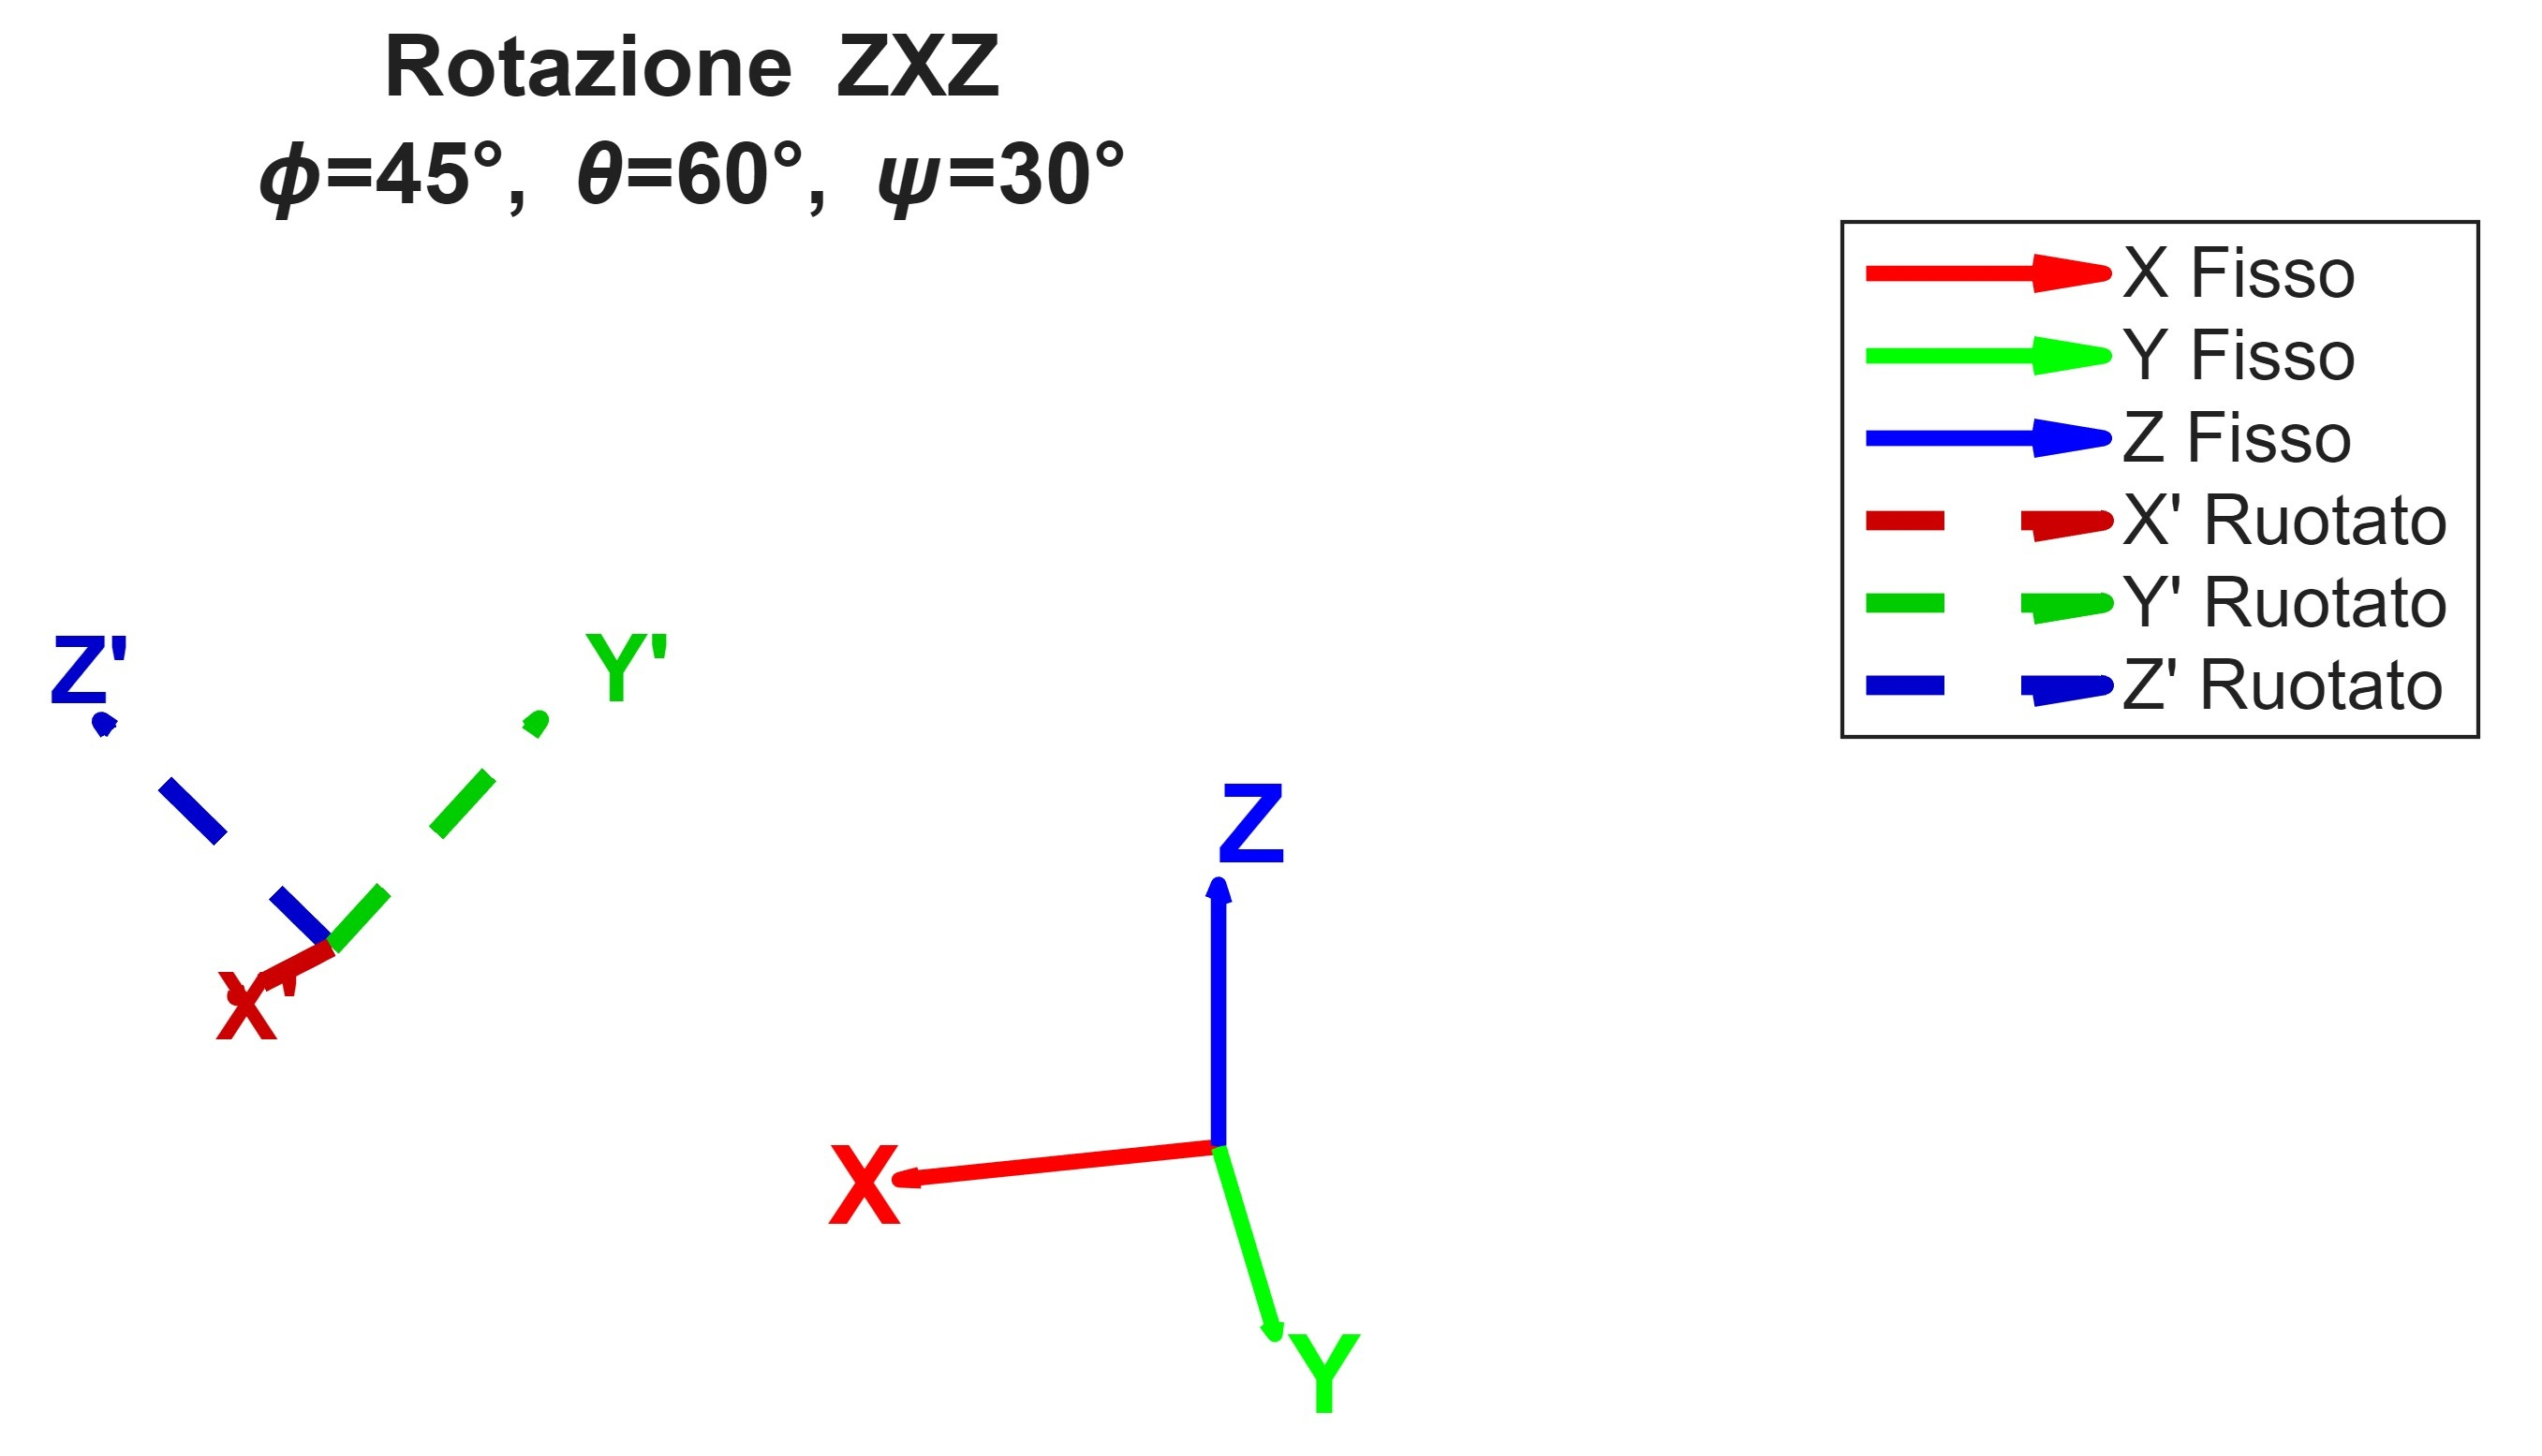
\includegraphics[width=1\linewidth]{figure_0.jpeg}
    \end{figure}
\end{center}
\matlabheadingtwo{\textbf{Visualizzazione Rotazione ZXY}}

\begin{matlabcode}
phiNum = pi/6;
thetaNum = pi/4;
psiNum = pi/3;

% Creazione Figura
figure('Name', 'Visualizzazione Rotazione ZXY');
hold on;

% Sistema di Riferimento Fisso
quiver3(0, 0, 0, 1, 0, 0, 'r', 'LineWidth', 2, 'DisplayName', 'X Fisso');
quiver3(0, 0, 0, 0, 1, 0, 'g', 'LineWidth', 2, 'DisplayName', 'Y Fisso');
quiver3(0, 0, 0, 0, 0, 1, 'b', 'LineWidth', 2, 'DisplayName', 'Z Fisso');
text(1.1, 0, 0, 'X', 'FontSize', 14, 'Color', 'r', 'FontWeight', 'bold');
text(0, 1.1, 0, 'Y', 'FontSize', 14, 'Color', 'g', 'FontWeight', 'bold');
text(0, 0, 1.1, 'Z', 'FontSize', 14, 'Color', 'b', 'FontWeight', 'bold');

% Estrazione Assi Ruotati
X_Ruotato = R_ZXY_Num(:, 1);
Y_Ruotato = R_ZXY_Num(:, 2);
Z_Ruotato = R_ZXY_Num(:, 3);

% Sistema di Riferimento Ruotato (ZXY)
quiver3(2.5, 0, 1, X_Ruotato(1), X_Ruotato(2), X_Ruotato(3), 'Color', [0.8 0 0], 'LineStyle', '--', 'LineWidth', 2.5, 'DisplayName', 'X'' Ruotato');
quiver3(2.5, 0, 1, Y_Ruotato(1), Y_Ruotato(2), Y_Ruotato(3), 'Color', [0 0.8 0], 'LineStyle', '--', 'LineWidth', 2.5, 'DisplayName', 'Y'' Ruotato');
quiver3(2.5, 0, 1, Z_Ruotato(1), Z_Ruotato(2), Z_Ruotato(3), 'Color', [0 0 0.8], 'LineStyle', '--', 'LineWidth', 2.5, 'DisplayName', 'Z'' Ruotato');
\end{matlabcode}
\newpage
\begin{matlabcode}
text(2.5 + X_Ruotato(1)*1.1, 0 + X_Ruotato(2)*1.1, 1 + X_Ruotato(3)*1.1, 'X''', 'FontSize', 14, 'Color', [0.8 0 0], 'FontWeight', 'bold');
text(2.5 + Y_Ruotato(1)*1.1, 0 + Y_Ruotato(2)*1.1, 1 + Y_Ruotato(3)*1.1, 'Y''', 'FontSize', 14, 'Color', [0 0.8 0], 'FontWeight', 'bold');
text(2.5 + Z_Ruotato(1)*1.1, 0 + Z_Ruotato(2)*1.1, 1 + Z_Ruotato(3)*1.1, 'Z''', 'FontSize', 14, 'Color', [0 0 0.8], 'FontWeight', 'bold');

% --- IMPOSTAZIONI STILE E VISUALIZZAZIONE FIGURA ---
title({'Rotazione ZXY', ['\phi=' num2str(rad2deg(phiNum)) '°, \theta=' num2str(rad2deg(thetaNum)) '°, \psi=' num2str(rad2deg(psiNum)) '°']});
legend('show', 'Location', 'northeastoutside');
grid off;
box off;
axis off;
axis equal;
rotate3d on;
view(-190, 16);

hold off;
\end{matlabcode}
\begin{center}
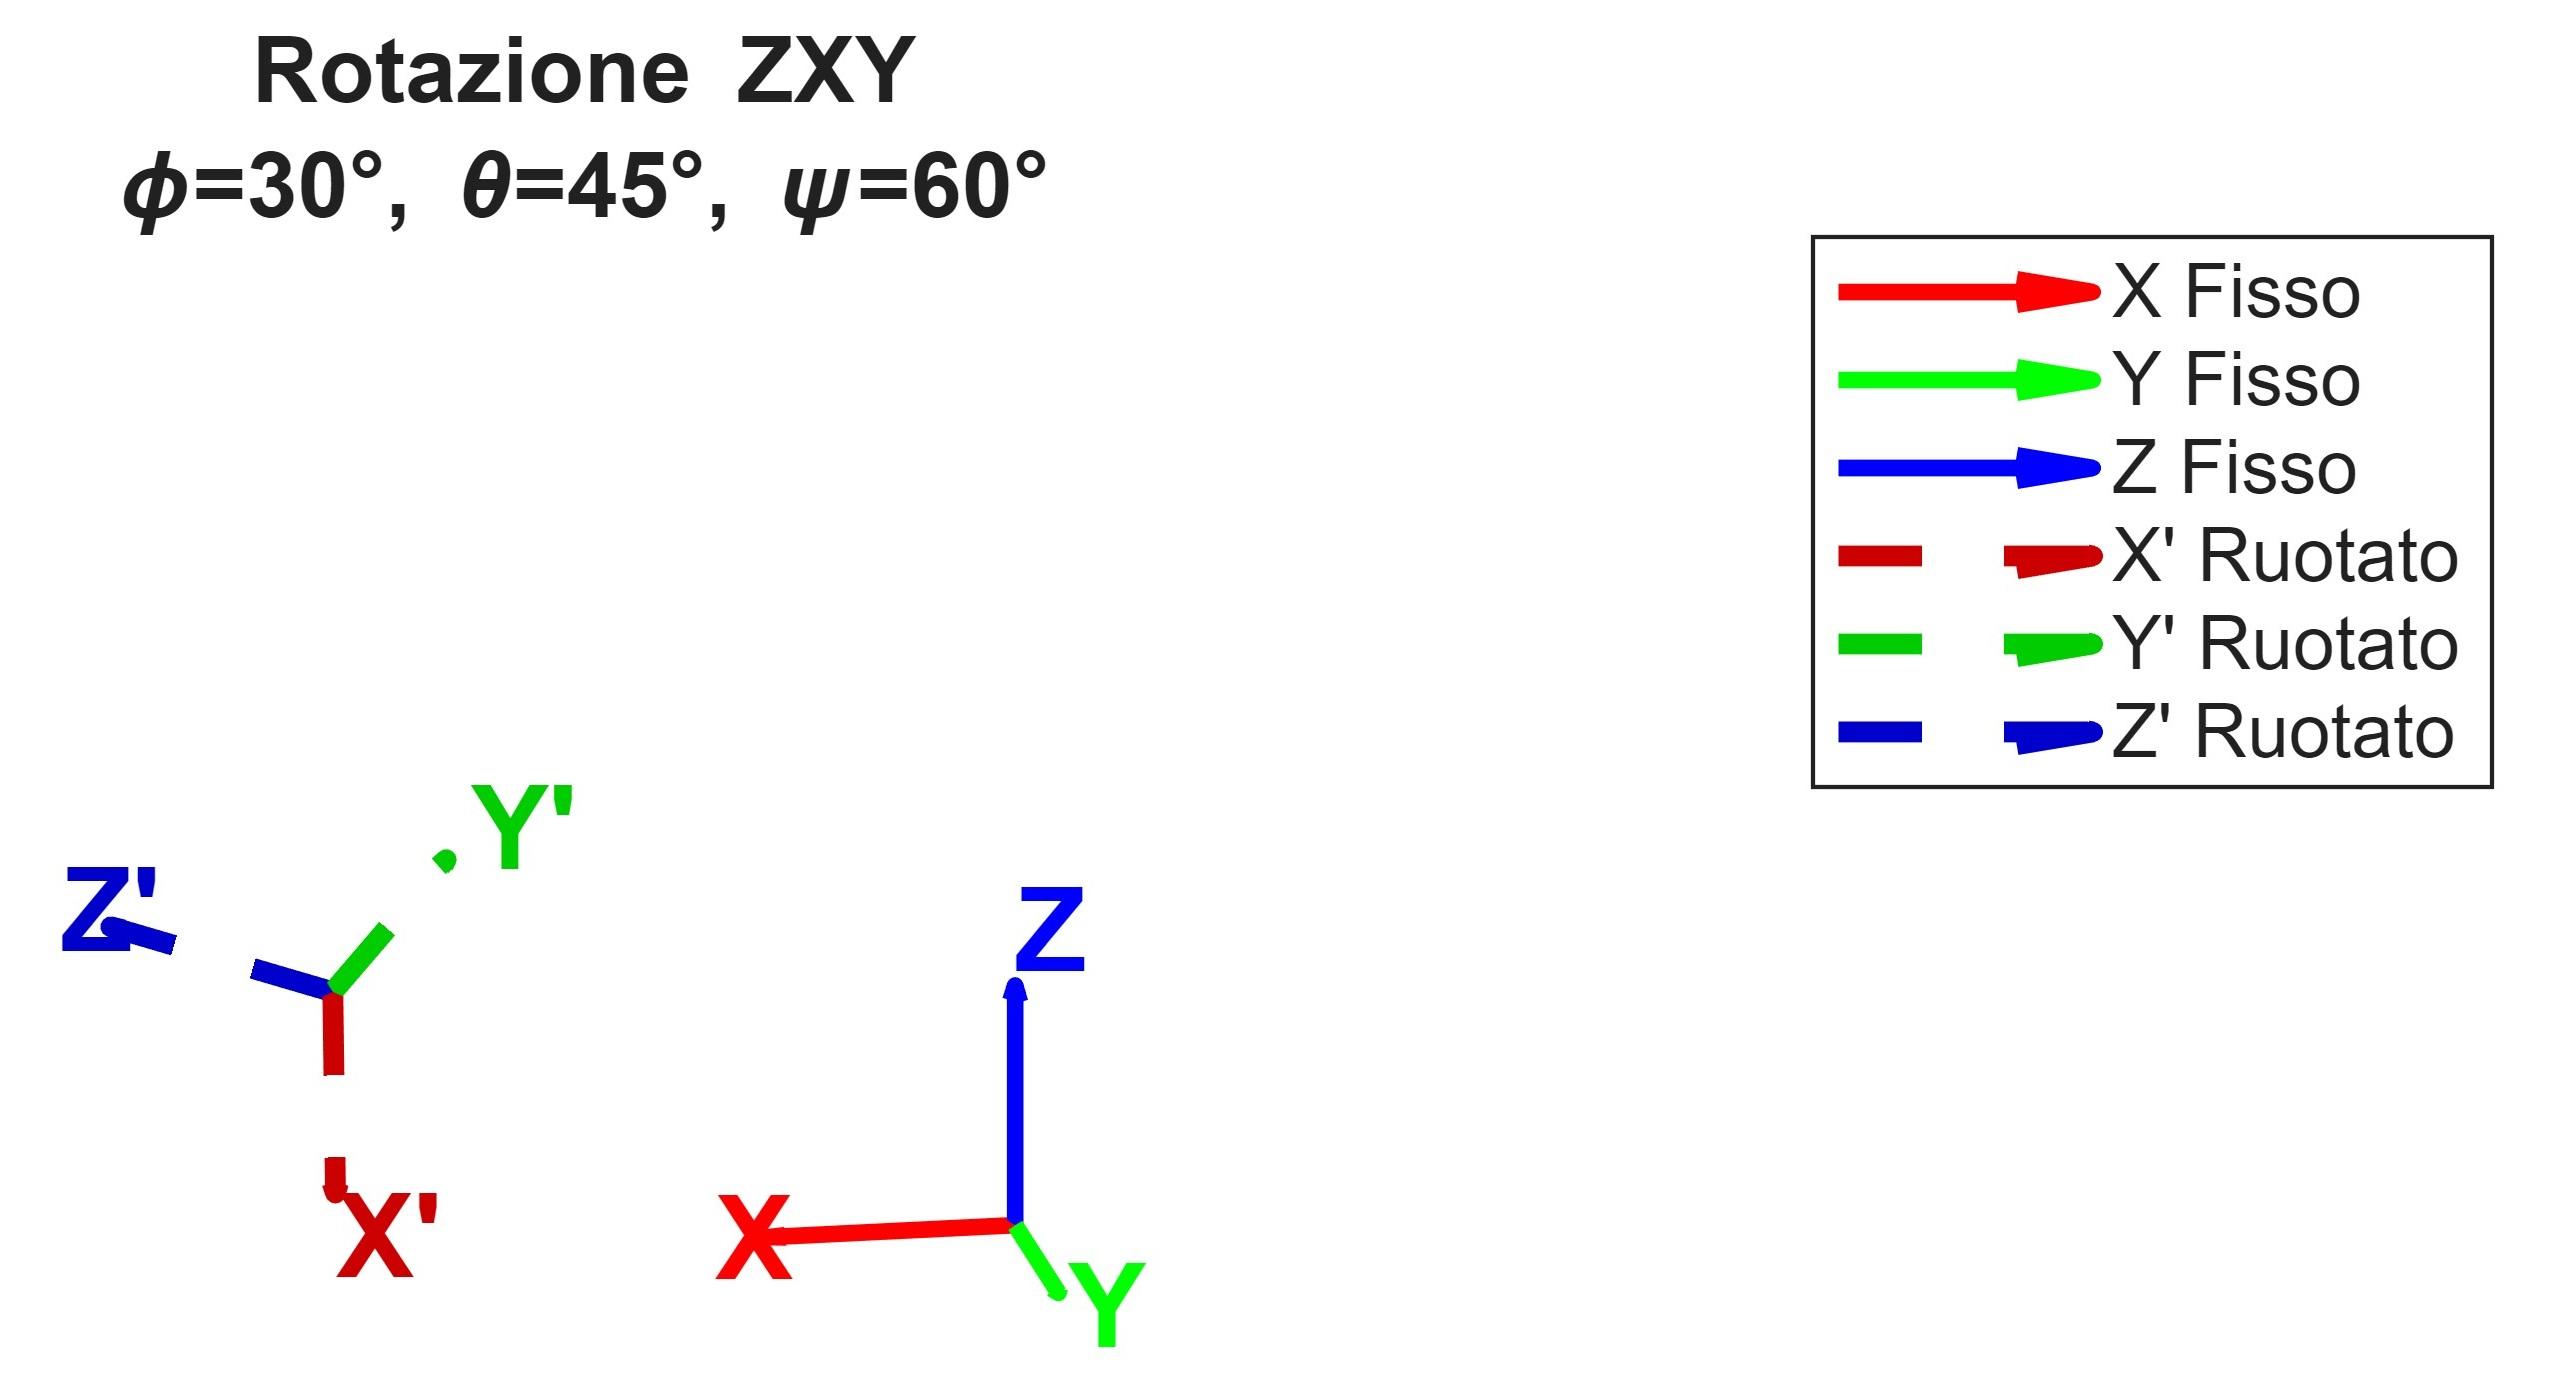
\includegraphics[width=1\linewidth]{figure_1.jpeg}
\end{center}

\matlabheadingtwo{\textbf{Visualizzazione Rotazione RPY}}

\begin{matlabcode}
% Creazione Figura
figure('Name', 'Visualizzazione Rotazione RPY');
hold on;

% Sistema di Riferimento Fisso
quiver3(0, 0, 0, 1, 0, 0, 'r', 'LineWidth', 2, 'DisplayName', 'X Fisso');
quiver3(0, 0, 0, 0, 1, 0, 'g', 'LineWidth', 2, 'DisplayName', 'Y Fisso');
quiver3(0, 0, 0, 0, 0, 1, 'b', 'LineWidth', 2, 'DisplayName', 'Z Fisso');
text(1.1, 0, 0, 'X', 'FontSize', 14, 'Color', 'r', 'FontWeight', 'bold');
text(0, 1.1, 0, 'Y', 'FontSize', 14, 'Color', 'g', 'FontWeight', 'bold');
text(0, 0, 1.1, 'Z', 'FontSize', 14, 'Color', 'b', 'FontWeight', 'bold');

% Estrazione Assi Ruotati
X_Ruotato = R_RPY_Num(:, 1);
Y_Ruotato = R_RPY_Num(:, 2);
Z_Ruotato = R_RPY_Num(:, 3);
\end{matlabcode}
\newpage
\begin{matlabcode}
% Sistema di Riferimento Ruotato (RPY)
quiver3(2.5, 0, 1, X_Ruotato(1), X_Ruotato(2), X_Ruotato(3), 'Color', [0.8 0 0], 'LineStyle', '--', 'LineWidth', 2.5, 'DisplayName', 'X'' Ruotato');
quiver3(2.5, 0, 1, Y_Ruotato(1), Y_Ruotato(2), Y_Ruotato(3), 'Color', [0 0.8 0], 'LineStyle', '--', 'LineWidth', 2.5, 'DisplayName', 'Y'' Ruotato');
quiver3(2.5, 0, 1, Z_Ruotato(1), Z_Ruotato(2), Z_Ruotato(3), 'Color', [0 0 0.8], 'LineStyle', '--', 'LineWidth', 2.5, 'DisplayName', 'Z'' Ruotato');
text(2.5 + X_Ruotato(1)*1.1, 0 + X_Ruotato(2)*1.1, 1 + X_Ruotato(3)*1.1, 'X''', 'FontSize', 14, 'Color', [0.8 0 0], 'FontWeight', 'bold');
text(2.5 + Y_Ruotato(1)*1.1, 0 + Y_Ruotato(2)*1.1, 1 + Y_Ruotato(3)*1.1, 'Y''', 'FontSize', 14, 'Color', [0 0.8 0], 'FontWeight', 'bold');
text(2.5 + Z_Ruotato(1)*1.1, 0 + Z_Ruotato(2)*1.1, 1 + Z_Ruotato(3)*1.1, 'Z''', 'FontSize', 14, 'Color', [0 0 0.8], 'FontWeight', 'bold');


% Impostazioni Figura
title({'Rotazione RPY (ZY''X'' - Yaw, Pitch, Roll)', ['\phi=' num2str(rad2deg(phiNum)) '°, \theta=' num2str(rad2deg(thetaNum)) '°, \psi=' num2str(rad2deg(psiNum)) '°']});
legend('show', 'Location', 'northeastoutside');
grid off;
box off;
axis off;
axis equal;
rotate3d on;
view(-190, 16);

hold off;
\end{matlabcode}
\begin{center}
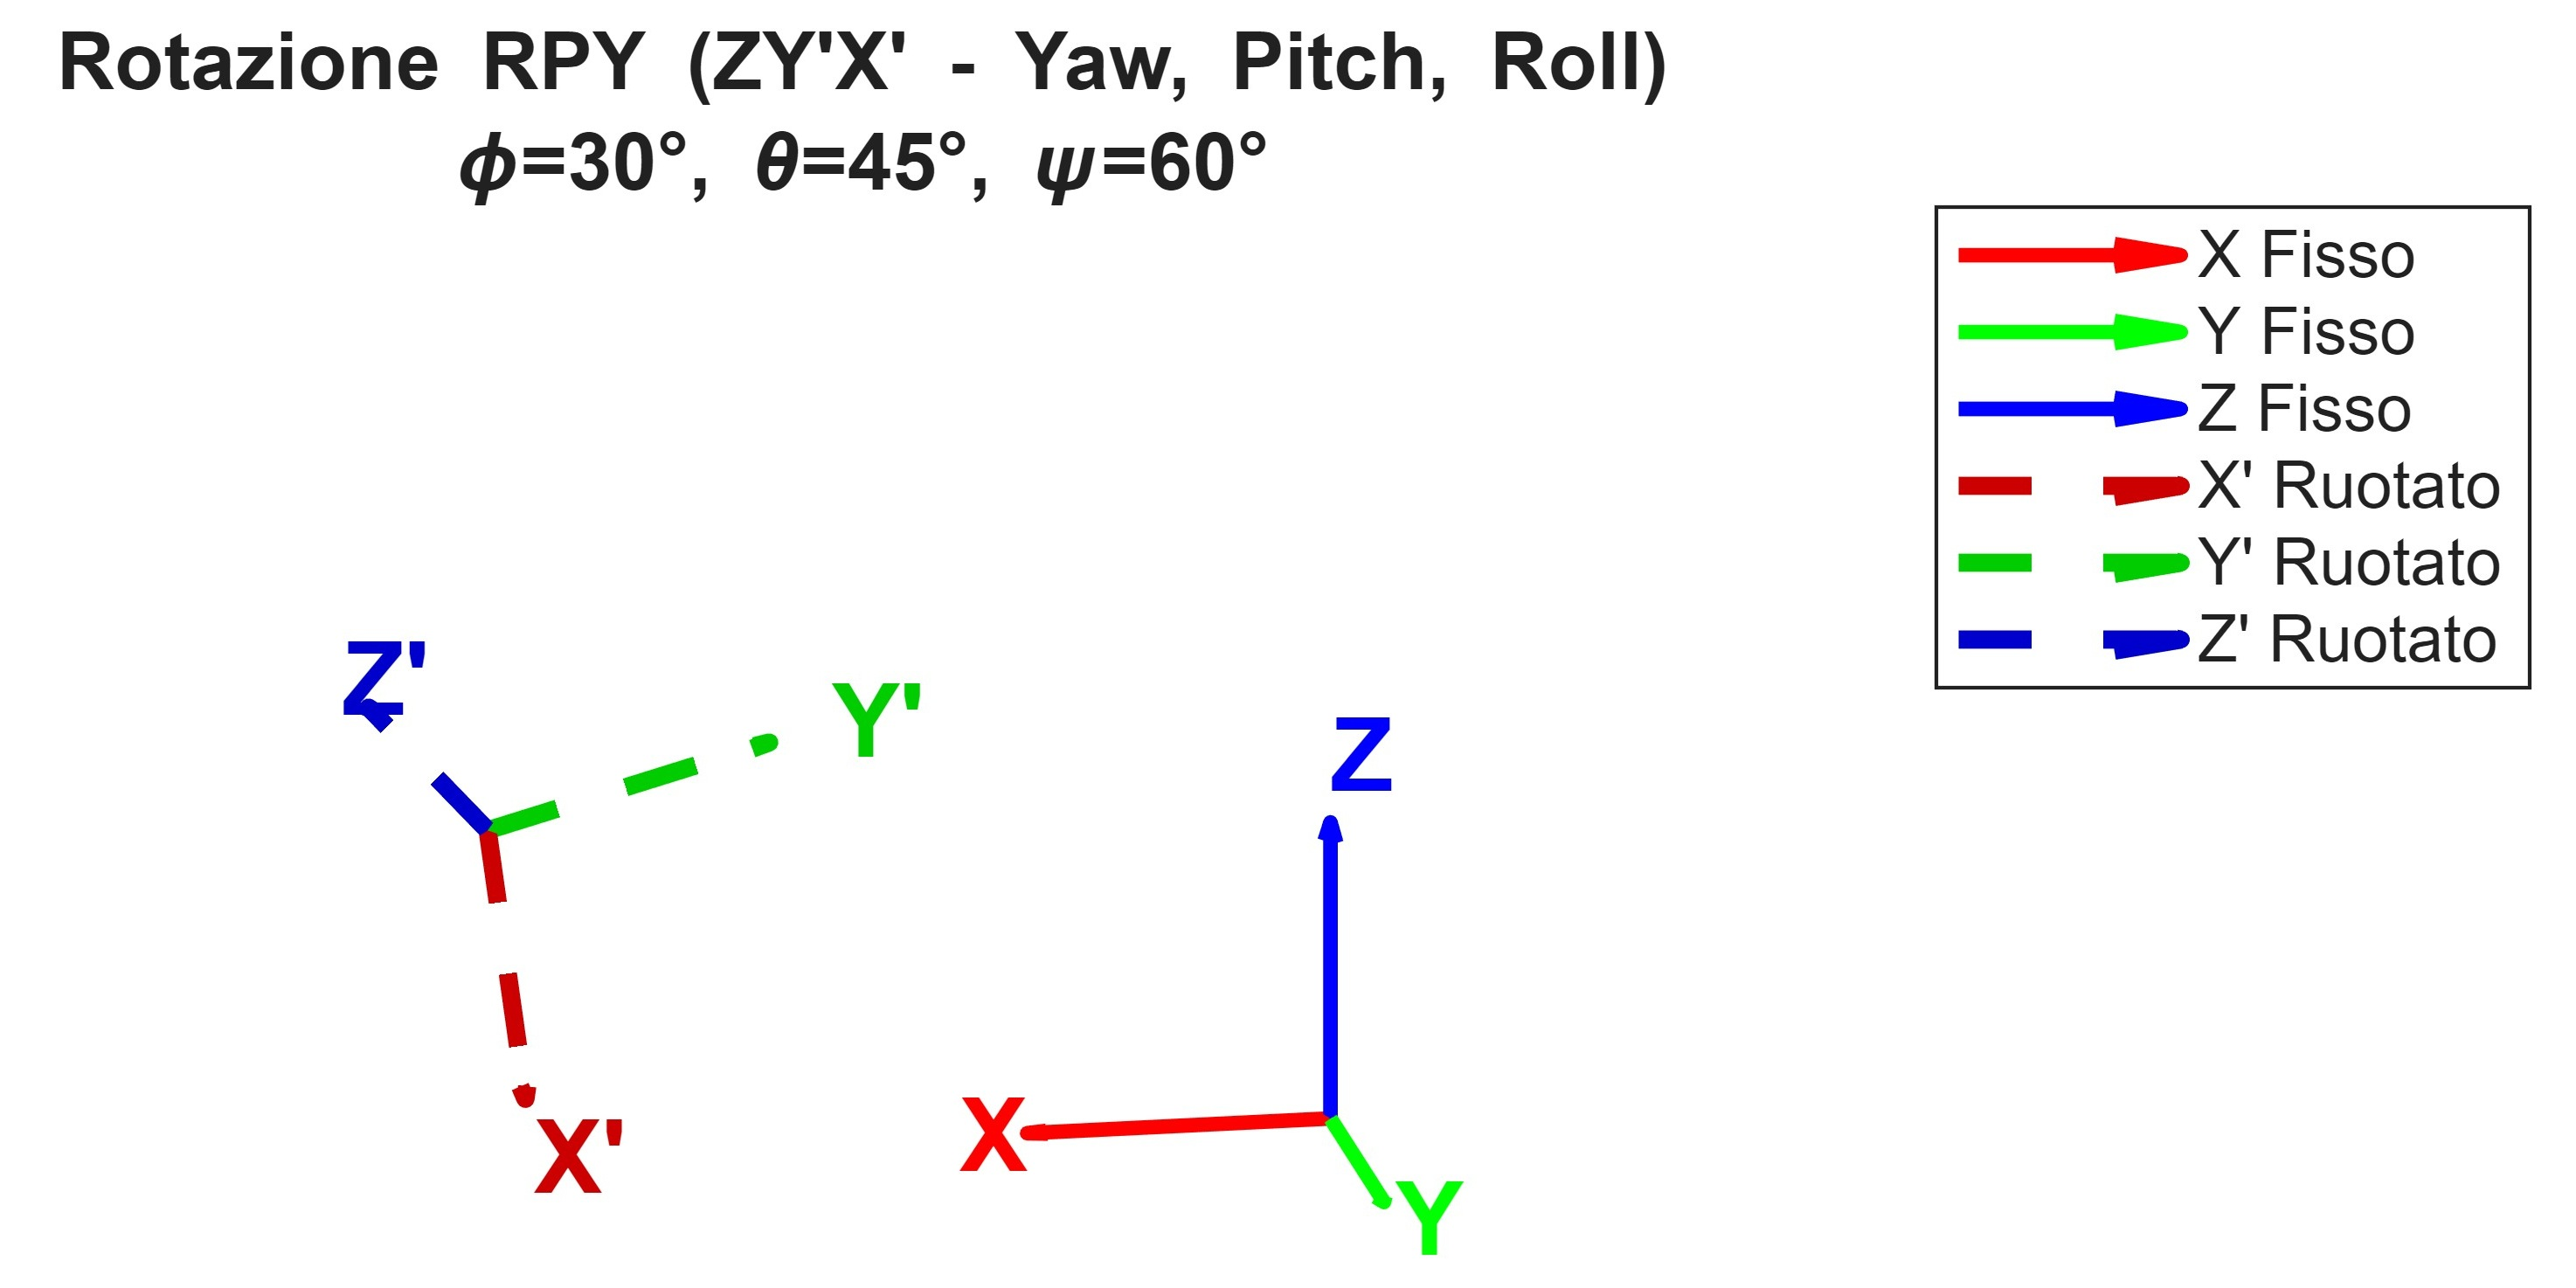
\includegraphics[width=1\linewidth]{figure_2.jpeg}
\end{center}


\end{document}
